\documentclass[tikz,border=3pt]{standalone}

\usepackage[T1]{fontenc}
\usepackage{libertine}
\usepackage{inconsolata}
\usepackage{newtxmath}
\usetikzlibrary{arrows.meta,calc}

\definecolor{graphink}{HTML}{263238}
\definecolor{orderfill}{HTML}{F5F1EA}
\definecolor{orderline}{HTML}{8C7256}
\definecolor{userfill}{HTML}{EEF4F7}
\definecolor{userline}{HTML}{557A8A}
\definecolor{relcolor}{HTML}{315F78}

\begin{document}
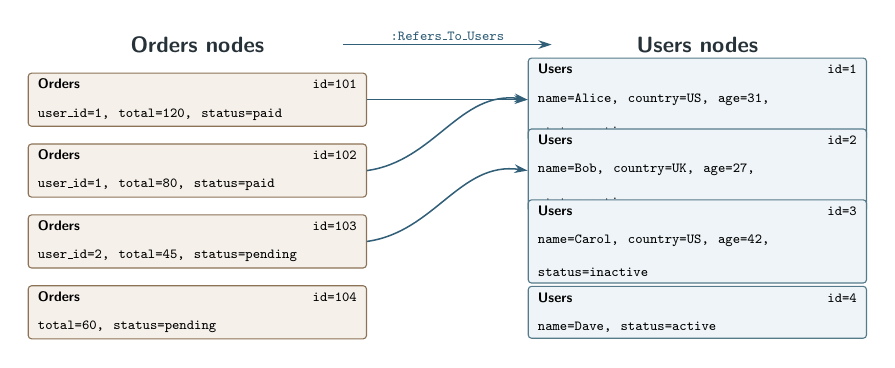
\begin{tikzpicture}[
  card/.style={
    draw=graphink!72,
    line width=0.4pt,
    rounded corners=1.2pt,
    text width=4.05cm,
    minimum height=0.58cm,
    inner xsep=3.5pt,
    inner ysep=2.2pt,
    align=left
  },
  order/.style={card, fill=orderfill, draw=orderline},
  user/.style={card, fill=userfill, draw=userline},
  heading/.style={font=\sffamily\bfseries\footnotesize, text=graphink},
  relationship/.style={
    -{Stealth[length=1.7mm,width=1.1mm]},
    draw=relcolor,
    line width=0.55pt
  },
  typekey/.style={
    font=\ttfamily\tiny,
    text=relcolor,
    fill=white,
    inner xsep=2pt,
    inner ysep=0.8pt
  }
]

\node[heading] at (0,2.05) {Orders nodes};
\node[heading] at (6.35,2.05) {Users nodes};
\draw[relationship] (1.85,2.05) --
  node[typekey,above=0.5pt] {:Refers\_To\_Users} (4.50,2.05);

\node[order] (o101) at (0,1.35)
  {\sffamily\bfseries\tiny Orders\hfill\ttfamily\tiny id=101\\[-1.8pt]
   \ttfamily\tiny user\_id=1, total=120, status=paid};
\node[order] (o102) at (0,0.45)
  {\sffamily\bfseries\tiny Orders\hfill\ttfamily\tiny id=102\\[-1.8pt]
   \ttfamily\tiny user\_id=1, total=80, status=paid};
\node[order] (o103) at (0,-0.45)
  {\sffamily\bfseries\tiny Orders\hfill\ttfamily\tiny id=103\\[-1.8pt]
   \ttfamily\tiny user\_id=2, total=45, status=pending};
\node[order] (o104) at (0,-1.35)
  {\sffamily\bfseries\tiny Orders\hfill\ttfamily\tiny id=104\\[-1.8pt]
   \ttfamily\tiny total=60, status=pending};

\node[user] (u1) at (6.35,1.35)
  {\sffamily\bfseries\tiny Users\hfill\ttfamily\tiny id=1\\[-1.8pt]
   \ttfamily\tiny name=Alice, country=US, age=31, status=active};
\node[user] (u2) at (6.35,0.45)
  {\sffamily\bfseries\tiny Users\hfill\ttfamily\tiny id=2\\[-1.8pt]
   \ttfamily\tiny name=Bob, country=UK, age=27, status=active};
\node[user] (u3) at (6.35,-0.45)
  {\sffamily\bfseries\tiny Users\hfill\ttfamily\tiny id=3\\[-1.8pt]
   \ttfamily\tiny name=Carol, country=US, age=42, status=inactive};
\node[user] (u4) at (6.35,-1.35)
  {\sffamily\bfseries\tiny Users\hfill\ttfamily\tiny id=4\\[-1.8pt]
   \ttfamily\tiny name=Dave, status=active};

\draw[relationship] (o101.east) -- (u1.west);
\draw[relationship] (o102.east) to[out=8,in=172] (u1.west);
\draw[relationship] (o103.east) to[out=8,in=172] (u2.west);

\end{tikzpicture}
\end{document}
